Gene networks are among the most crucial frameworks to study in biological research today.
These methods have evolved from their first application of network science in genomic biology and are combined with ecological models to improve performance metrics like accuracy and interpretability over time.

Traditionally, the origins of network analysis in science go back as far as 1736 when Leonhard Euler solved the Seven Bridges of Königsberg (\autoref{fig:seven-bridges-of-königsberg}) problem that enabled development of graph theory and its applications\cite{euler_solutio_1726}.
The challenge posed to Euler was deceptively simple: Could a person cross all seven bridges exactly once without retracing their steps?
Euler approached this problem by abstracting the geography of Königsberg into a network of nodes and edges.
The landmasses were represented as nodes, and the bridges connecting them were represented as edges.
% insert a image
\begin{figure}[h!]
    \centering
    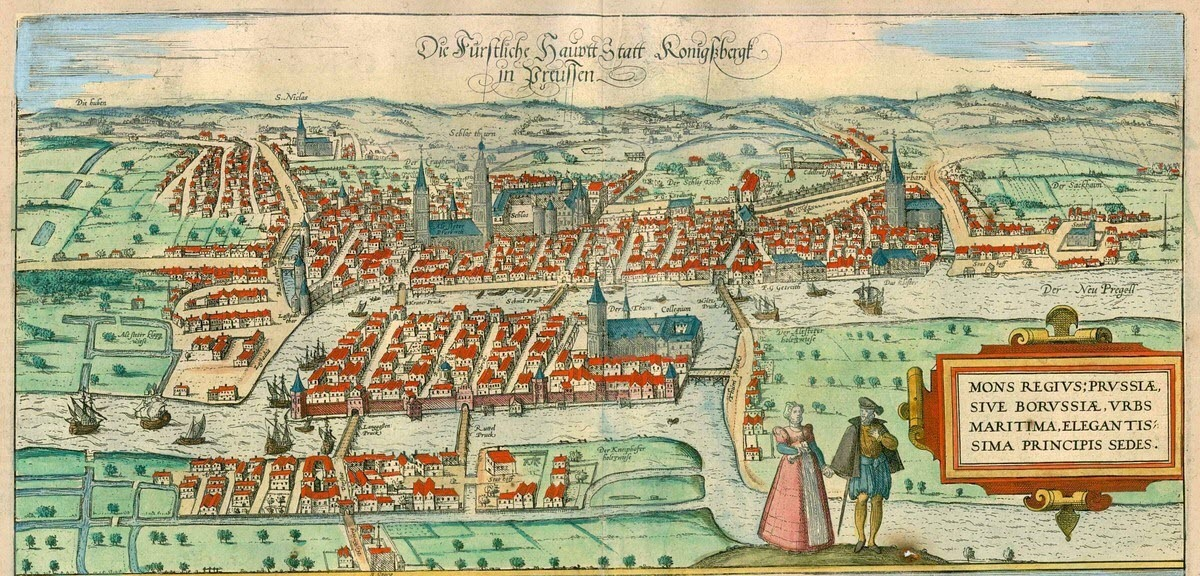
\includegraphics[width=0.75\textwidth]{konigsberg-1581-22} % Path to your image file
    \caption{Seven Bridges of Königsberg\cite{young_seven_2020}}
    \label{fig:seven-bridges-of-königsberg}
\end{figure}

\noindent Euler proved that the problem had no solution, laying down two key principles in the process:
\begin{enumerate}
    \item Nodes and Edges: Euler identified that the ability to traverse a network depends on the degree of each node (the number of edges connected to it).
    For a path that crosses each edge exactly once (an Eulerian path), all but two nodes must have an even degree.
    \item Graph Connectivity: The network must be connected, meaning all nodes must be reachable from any other node.
\end{enumerate}

\noindent In the case of Königsberg, all four nodes had an odd degree, making it impossible to traverse the network under the stated conditions.
This conclusion not only resolved the Königsberg problem but also established the first theorem of graph theory.
\\\\
Jacob Moreno and Helen Jennings took this idea a step further in the 1930s, drawing social relationships with sociometric maps that would be some of the first systematic applications of network analysis to social science\cite{moreno_who_1934}.
Use of network analysis has been applied to other domains like physics\cite{kirchhoff_solution_1958} and chemistry\cite{arthur_mathematical_1896}, showing how versatile and hwo impactful this field can be.
This is why, in this work, the evolution of gene network analysis will be discussed, with a particular focus on the use of Random Matrix Theory (RMT) to increase robustness during network construction.


Gene networks are intricate representations of interactions among genes and their products within biological systems\cite{oldham_conservation_2006}.
These networks, composed of nodes symbolizing genes and edges reflecting interactions\cite{barabasi_network_2004}, offer a system-wide perspective on cellular processes.
Researchers leverage these networks to investigate critical biological phenomena\cite{barabasi_network_2004}, such as development\cite{montoya_ecological_2006}, disease progression\cite{friedman_using_2000}, and evolutionary adaptations\cite{dunne_food-web_2002}.
Notably, gene networks are instrumental in identifying gene modules—highly connected clusters of genes that frequently correspond to functional units and hub genes, which play pivotal roles in maintaining cellular integrity\cite{zhang_general_2005}.
\\\\
The construction of gene networks uses diverse methodologies.
Equation-based models, for instance, infer gene interactions from differential equations that describe gene expression dynamics\cite{deng_molecular_2012}.
Bayesian approaches, on the other hand, use probabilistic models to estimate gene interactions based on prior knowledge and observed data\cite{gerstung_quantifying_2009}.
Co-expression networks are another prevalent approach, they use correlation matrices derived from gene expression data to identify links between genes that exhibit strong statistical relationships\cite{zhang_general_2005}.
These approaches often rely on determining appropriate thresholds to distinguish meaningful biological connections from random noise, a process that remains subjective and heavily influenced by prior knowledge or statistical frameworks.
Despite their utility, traditional network approaches face challenges such as scalability and sensitivity to noise, emphasizing the need for advanced methods to refine and automate the thresholding process\cite{deng_molecular_2012}.
\\\\
This bibliography takes you on a journey through the history of methods for analyzing gene networks, with particular focus on the game-changing application of RMT in providing greater robustness to network construction.
This work highlights the need for such advanced methods as well as the integration of approaches like co-expression networks in frameworks such as the Molecular Ecological Network Analysis Pipeline (MENAP) that aim to capture complex biological architectures.